% !TEX root = main.tex
% Loomstead paper draft entry. Keep the file lightweight until the citation flow is ready.
\documentclass[11pt]{article}

\usepackage[margin=1in]{geometry}
\usepackage{booktabs}
\usepackage{hyperref}

\hypersetup{
  colorlinks=true,
  linkcolor=blue,
  citecolor=blue,
  urlcolor=blue
}

\title{Loomstead: Motivational Delegation for Process-Constrained Goals in Persistent Multi-Agent Narratives}
\author{Draft workspace}
\date{May 2026}

\begin{document}
\maketitle

\begin{abstract}
Persistent multi-agent narratives often involve goals whose value lies in the path taken. Friendships should grow through shared events, trust repair should depend on remembered harm and observed compensation, and festivals should succeed through visible social and resource processes. Loomstead studies motivational delegation: a Director shapes conditions through motivation bias, opportunity scheduling, information exposure, event pressure, and constraints while autonomous NPC agents choose actions through their own motivation, memory, relationships, and heuristics. The system pairs a playable Godot town slice with a Python runtime, traceable tool execution, subjective memory, relationship edges, and Process Fidelity Eval. Current evidence is a research-preview scaffold built from rule-level process scenarios, hard-delegation and memory ablations, stability runs, and a small cross-domain coding adapter.
\end{abstract}

\section{Introduction}

Persistent multi-agent narrative systems need to handle goals whose success depends on visible intermediate processes. A relationship should improve because characters shared events, remembered them, and later acted differently. A festival should succeed through resource pressure, social participation, and divergent subjective memories. Loomstead frames this problem as process-constrained goal achievement.

The central mechanism is motivational delegation. A Director may bias motivations, expose information, create opportunities, load event pressure, shift resources, or inject constraints. NPCs still select actions through their own needs, memories, relationships, heuristics, and tool capabilities. The research question is whether this pattern can produce traceable progress toward user goals while preserving autonomy and process fidelity.

This draft currently makes three scoped contributions:

\begin{enumerate}
  \item A runtime pattern for motivational delegation in a persistent narrative town slice.
  \item A Process Fidelity Eval suite with shortcut, autonomy, memory-causality, and trace-coverage metrics.
  \item A manifest-backed evidence workflow for connecting runtime traces, ablations, stability runs, and paper claims.
\end{enumerate}

\section{Related Work}

\subsection{Believable generative agents}

Generative Agents introduced a small-town sandbox where LLM-driven agents retrieve memories, reflect, plan, and produce believable social behavior~\cite{park2023generativeAgents}. Concordia generalizes this style of generative agent-based modeling through grounded environments, associative memory, and a Game Master that mediates agent actions into environment effects~\cite{vezhnevets2023concordia}. Loomstead builds on the same broad motivation: persistent agents should have memory and socially legible behavior. Its narrower research target is goal-conditioned orchestration. The Director receives process-constrained goals, applies indirect interventions, and exports evidence about whether the resulting social process respected autonomy, memory causality, and traceability.

\subsection{Drama management and authorial control}

Interactive narrative research has long studied the tension between authorial goals and user or character autonomy. Drama-management surveys describe drama managers as coordinators that influence narrative experience while reasoning about authorial intent, player actions, and qualitative story objectives~\cite{roberts2008dramaManagementSurvey}. Loomstead connects this theme to modern multi-agent runtimes by making the intervention boundary explicit. Director actions are limited to motivation bias, opportunity scheduling, information exposure, resource shifts, event pressure, constraints, and checkpoints. The evaluation then asks whether these interventions created an earned process, whether NPC actions remained agent-initiated, and whether key state changes can be traced through events and memories.

\subsection{Task-oriented multi-agent orchestration}

AutoGen provides customizable conversable agents for LLM applications, including human, tool, and LLM-backed interaction modes~\cite{wu2023autogen}. MetaGPT encodes standard operating procedures into role-based prompt sequences for collaborative software work~\cite{hong2024metagpt}. ChatDev organizes specialized software-development agents through a chat chain and communicative dehallucination~\cite{qian2024chatdev}. These systems are important references for explicit workflow decomposition and task delegation. Loomstead treats that family as a useful contrast class for narrative goals: a direct assignment can achieve an end state while increasing forced-action and shortcut rates. The paper's secondary coding adapter uses software fixtures only as a portability check for GoalSpec, trace, and eval abstractions.

\subsection{Agent evaluation}

AgentBench evaluates LLM agents across interactive environments and emphasizes decision-making ability in multi-turn settings~\cite{liu2024agentbench}. Loomstead adopts the interactive-evaluation spirit, then focuses the target on process-constrained social goals. Current metrics include goal success, shortcut violation rate, required process coverage, forced-action rate, agent-initiated action ratio, relationship-memory causal use, causal trace coverage, and process believability. The related-work gap is therefore methodological: how to evaluate an agent society when the final state is insufficient and the explanatory process is part of the claim.

The live literature review remains in \texttt{paper/lit\_review/}. The current citation set is a seed list and still needs trace-debugging, human believability, and game-AI social simulation sources.

\section{System Overview}

Loomstead uses a Godot client for the playable town slice and a Python Agent Server for authoritative world state. The client presents player movement, visual-novel feedback, NPC map state, event visualization, and the Phase 2 observer panel. The server owns world simulation, legal tool execution, Director beats, Event Skills, NPC motivation, capability filtering, arbitration, subjective memory, relationship edges, heuristic learning, provider routing, debug traces, and eval export.

\begin{figure}[t]
\centering
\fbox{\begin{minipage}{0.92\linewidth}
\small
\textbf{Figure source:} \texttt{paper/diagrams/system\_overview.mmd}.\\[0.4em]
\textbf{Client:} Godot town slice, visual feedback, observer panel.\\
\textbf{Server:} Director / Event Skill, NPC loop, ToolExecutor, memory stores, schema registry.\\
\textbf{Evidence path:} trace events and manifests flow into Debug UI, Process Fidelity Eval, and paper tables.
\end{minipage}}
\caption{Loomstead runtime overview. The committed Mermaid source is the editable figure draft; this boxed version keeps the LaTeX scaffold self-contained until rendered assets are produced.}
\label{fig:system-overview}
\end{figure}

Figure~\ref{fig:system-overview} summarizes the current runtime boundary. The Godot client reads state through server APIs and submits legal player actions. The Python Agent Server remains the only authoritative writer for world state. LLM or rule-provider outputs enter visible gameplay through parsing, validation, fallback, tool execution, event recording, and trace export.

\subsection{Authoritative world and tool execution}

World state updates pass through runtime tools and avoid ad hoc state edits. The ToolDefinition registry and CapabilityRegistry filter available tools by need relevance, preconditions, NPC profile, event scope, and budget policy. ToolExecutor records sustained action state, transaction snapshots, completion events, failure events, rollback evidence, and interruption traces. This path gives the eval layer a stable place to detect illegal shortcuts and forced actions.

\subsection{NPC decision loop}

At each tick, NeedAccumulator computes candidate needs from NPC status and content data. CapabilityRegistry resolves legal candidate tools. ArbitrationLayer scores candidates using motivation, relationship edges, recalled subjective memories, and active heuristics. The selected action is therefore tied to a traceable set of contributing sources. The current Phase 2 runtime exposes this path through \texttt{motivation.decision\_made}, then follows the selected tool through completion, failure, interruption, and observation events.

\subsection{Memory, relationship, and heuristic stores}

The memory layer separates objective events from subjective observations. ResultObserver and BiasFilter convert visible tool results into per-NPC subjective memories. RelationshipEdgeStore tracks relationship deltas with source references. HeuristicLibrary records learned or designer-seeded preferences such as successful tools, interrupted tools, and social-affiliation rules. These stores feed later arbitration, giving the paper a concrete mechanism for claims about memory causality and relationship-conditioned behavior.

\subsection{Debug and eval contract}

Schema versions are centralized through \texttt{schema\_registry.v1}. The debug endpoint exposes decision, tool, interruption, memory, observer, and budget snapshots. Eval exports include manifests with artifact hashes, Git state, schema snapshots, metric ids, baselines, and scenario ids. The paper workflow reads those manifests into generated Markdown, CSV, JSON, and LaTeX tables, keeping prose claims linked to repository evidence.

\section{Motivational Delegation}

Motivational delegation is the paper's proposed runtime pattern for process-constrained narrative goals. A user or designer supplies a GoalSpec with a desired outcome, forbidden shortcuts, required process predicates, allowed interventions, and success evidence. The Director then selects interventions that change the action distribution of the world while leaving final action choice to NPC arbitration.

\begin{figure}[t]
\centering
\fbox{\begin{minipage}{0.92\linewidth}
\small
\textbf{Figure source:} \texttt{paper/diagrams/motivational\_delegation\_loop.mmd}.\\[0.4em]
GoalSpec $\rightarrow$ Director intervention $\rightarrow$ NPC motivation / opportunity / information / constraint context $\rightarrow$ arbitration-selected tool $\rightarrow$ objective event $\rightarrow$ subjective memory and relationship evidence $\rightarrow$ eval checkpoint.
\end{minipage}}
\caption{Motivational Delegation loop. The Director changes conditions and checkpoints progress; NPCs choose concrete actions through the normal runtime loop.}
\label{fig:motivational-delegation}
\end{figure}

Figure~\ref{fig:motivational-delegation} shows the loop. The Director may apply motivation bias, event-skill loading, opportunity scheduling, resource shifts, information exposure, constraint injection, and evaluation checkpoints. These interventions are explicit, traceable, and time-bounded. Prohibited intervention fields include direct final relationship state updates, concrete action assignments to specific NPCs, unobserved subjective memory injection, and ToolExecutor bypasses.

\subsection{GoalSpec}

A process-constrained GoalSpec contains five groups of data:

\begin{enumerate}
  \item \textbf{Desired outcome}: the final state or evidence condition that should hold.
  \item \textbf{Forbidden shortcuts}: state changes that would make the outcome unearned.
  \item \textbf{Required process}: predicates over shared events, memories, relationship evidence, and later decisions.
  \item \textbf{Allowed interventions}: the Director actions permitted for this goal.
  \item \textbf{Success evidence}: trace artifacts required before the run counts as successful.
\end{enumerate}

For example, a close-friend goal can require at least two positive shared events, subjective memories for both agents, relationship-edge source references, and a future behavior that references one of those memories. The same final relationship score without these artifacts should fail Process Fidelity Eval.

\subsection{Director intervention boundary}

The intervention boundary is the main design choice. The Director is allowed to alter world conditions that make certain actions more likely or more salient. It can schedule a gathering, expose a rumor to one NPC, raise the salience of a social need, constrain access to a shortcut, or load an Event Skill that creates localized pressure. The NPC loop still decides whether an NPC acts, what tool it uses, and how it reacts to success, failure, or interruption.

This boundary also makes Hard Delegation a meaningful baseline. In Hard Delegation, the Director translates the goal into assigned tasks for specific NPCs. In Full Motivational Delegation, the Director manipulates motivation and opportunity while the NPC's normal arbitration path remains active. Comparing these settings lets the paper measure whether final goal success came with forced actions, shortcut violations, weak process coverage, or missing memory evidence.

\subsection{Evidence lifecycle}

Each intervention should move through an evidence lifecycle:

\begin{enumerate}
  \item \textbf{Proposed}: the Director creates an intervention from the GoalSpec and world digest.
  \item \textbf{Applied}: validation checks the intervention type, scope, and allowed fields.
  \item \textbf{Observed}: NPC actions and tool outcomes create objective events.
  \item \textbf{Internalized}: eligible agents store subjective memories or relationship updates.
  \item \textbf{Reused}: later arbitration cites memories, relationship edges, or heuristics.
  \item \textbf{Evaluated}: Process Fidelity Eval checks goal success, process predicates, autonomy, and trace coverage.
\end{enumerate}

The lifecycle is deliberately audit-oriented. It gives the debug UI and paper tables a shared explanation path from intervention to outcome.

\section{Process Fidelity Eval}

Process Fidelity Eval measures whether goal progress follows a credible multi-agent process. A run succeeds only when the desired outcome and the required evidence chain are both satisfied. For a relationship goal, that evidence chain may include shared events, subjective memories for both agents, relationship-edge source references, and a later decision that cites a relevant memory or relationship edge.

\begin{figure}[t]
\centering
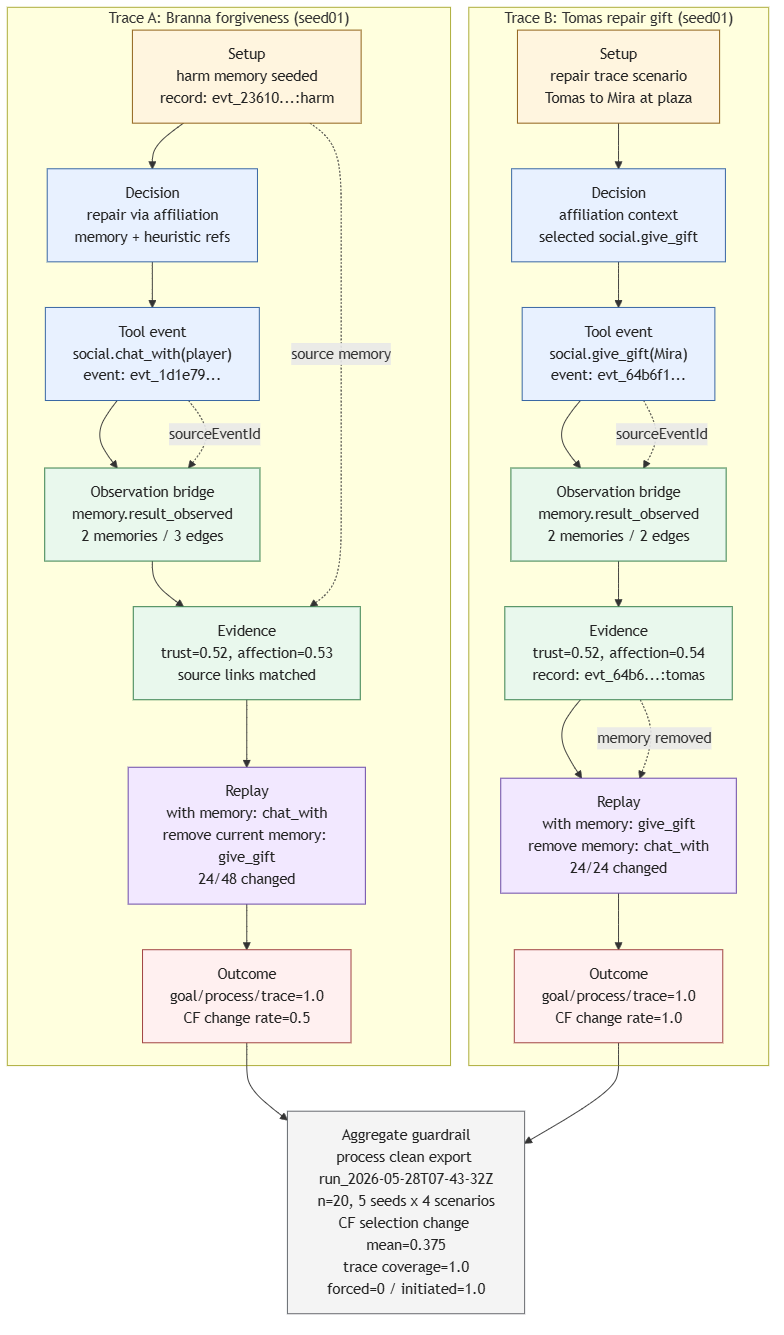
\includegraphics[width=\linewidth,height=0.72\textheight,keepaspectratio]{../generated/figures/trace_evidence_chain_figure3.png}
\caption{Trace evidence chains for two process-fidelity examples from the current clean process export, with an aggregate process-suite guardrail annotation. The editable Mermaid source at \texttt{paper/diagrams/trace\_evidence\_chain\_figure3.mmd} uses curated labels from process artifacts rather than raw event-summary text.}
\label{fig:trace-evidence-chain}
\end{figure}

\begin{table}[t]
\centering
\small
\caption{Process Fidelity metric families used by the current draft.}
\label{tab:metric-families}
\begin{tabular}{lll}
\toprule
Family & Example metrics & Question answered \\
\midrule
Outcome & goal success, milestones & Did the run satisfy the stated goal evidence? \\
Process & process coverage, shortcuts & Did the required path occur without illegal jumps? \\
Autonomy & forced action, agent initiation & Did NPC arbitration choose the relevant actions? \\
Memory & causal use, ablation delta & Did remembered events affect later decisions? \\
Trace & trace coverage, source links & Can the causal chain be replayed from artifacts? \\
Side effects & spillover, overreach & Did intervention cause uncontrolled collateral change? \\
\bottomrule
\end{tabular}
\end{table}

The current baseline matrix includes Full Motivational Delegation, Hard Delegation, No Subjective Memory, No Relationship Edge, Shuffled Memory Owner, and Evidence-Link Removal. Hard Delegation represents the explicit worker-agent pattern: a Director decomposes the goal into assigned subtasks and gives them to specific NPCs. The memory and evidence-link ablations test whether relationship memory is causally useful, whether the correct owner of a memory matters, and whether traces still justify relationship changes after source links are removed.

All current exported results should be read as scaffolding evidence. The metrics are already wired to manifests and generated paper tables, yet stronger research claims need repeated seeds, LLM-backed provider runs, runtime-level ablations, and human process-believability ratings.

\section{Evidence Skeleton}

This section stays at a research-preview evidence level. The current clean exports are \texttt{run\_2026-05-28T07-43-32Z} (process fidelity) and \texttt{domain\_2026-05-28T07-49-46Z} (cross-domain adapter), both with clean git manifests (\texttt{dirty=false}) at \texttt{b1c006f}. Generated paper tables under \texttt{paper/generated/} are treated as build guards and claim placeholders, and the prose keeps an interface-evidence scope.

\subsection{Process-fidelity ablations}

Table~\ref{tab:process-ablation} summarizes \texttt{run\_2026-05-28T07-43-32Z}, which exports 4 scenarios $\times$ 6 baselines $\times$ 5 seeds (120 per-scenario artifacts) with a stable schema and checksum-indexed manifest. At this stage, the table is used as local guardrail evidence for metric wiring and ablation surface integrity. The observed separations between full motivational delegation and ablated settings are reported as preview signals for process-fidelity instrumentation, and they are not promoted to final causal claims. Figure~\ref{fig:trace-evidence-chain} is drafted from the same clean export, using two curated per-scenario trace lanes plus an aggregate guardrail annotation.

\subsection{Stability runs}

Table~\ref{tab:stability-24h} reports the latest rule-level stability window and serves as regression guardrails for tick success, tool failures, interruptions, memory observations, and heuristic references. This evidence remains local scaffolding; publication-level claims still need repeated windows under matched runtime settings and explicit external-validity checks.

\subsection{Cross-domain adapter}

Table~\ref{tab:domain-adapter} reports \texttt{domain\_2026-05-28T07-49-46Z}, which contains deterministic five-seed exports over 11 scenarios (3 town + 8 coding dry-run fixtures) and passes 55/55 local checks. The adapter evidence is intentionally contract-level: it checks whether GoalSpec, trace envelopes, artifact manifests, replay exports, and summary metrics stay comparable while Loomstead town remains the primary validation surface. The coding rows verify fixture plumbing (snapshots, dependency graphs, patches, review reports, reviewer-arbitration traces, and counterfactual replay artifacts); they do not support claims about real-world coding-task performance. The current CF route means (coding \texttt{0.762}, town \texttt{0.333}) are reported as route-sensitivity instrumentation, not as human-believability or task-performance scores.

% Generated by scripts/paper_extract_eval_tables.py.
% Refresh with `npm.cmd run paper:tables` or `npm.cmd run paper:check`.

\begin{table}[t]
\centering
\small
\caption{Process Fidelity ablation summary from the latest local rule-level process suite. Lower is better for shortcut and forced-action rates; higher is better for the other metrics.}
\label{tab:process-ablation}
\begin{tabular}{lrrrrrrrr}
\toprule
Baseline & Goal & Process & Shortcut & Forced & Agent-init. & Memory & Trace & Believ. \\
\midrule
Full & 1 & 1 & 0 & 0 & 1 & 1 & 1 & 1 \\
Hard & 1 & 0.186 & 1 & 1 & 0 & 0 & 0 & 0.0371 \\
No memory & 1 & 0.743 & 0 & 0 & 1 & 1 & 1 & 0.949 \\
No relation & 0 & 0.814 & 0 & 0 & 1 & 0 & 0 & 0.563 \\
Shuffled owner & 0 & 0.814 & 0 & 0 & 1 & 0 & 1 & 0.763 \\
No evidence link & 0 & 0.814 & 1 & 0 & 1 & 0 & 0 & 0.363 \\
\bottomrule
\end{tabular}
\end{table}

\begin{table}[t]
\centering
\small
\caption{Stability metrics from the latest 24-hour local rule-level run.}
\label{tab:stability-24h}
\begin{tabular}{lrrr}
\toprule
Metric & Mean & Std. & N \\
\midrule
Tick success & 1 & 0 & 24 \\
Memory obs. & 1 & 0 & 1 \\
Tool fail & 0 & 0 & 1 \\
Interrupt & 0.143 & 0 & 1 \\
Heuristic ref. & 0.694 & 0 & 1 \\
\bottomrule
\end{tabular}
\end{table}

\begin{table}[t]
\centering
\small
\caption{Cross-domain adapter suite summary from the latest local dry-run fixtures. Repeats are deterministic export repeats, and CF route reports counterfactual tool-selection change rate.}
\label{tab:domain-adapter}
\begin{tabular}{lrrrrr}
\toprule
Domain & Passed & Total & Scenarios & Det. repeats & CF route \\
\midrule
loomstead.coding.v0 & 16 & 16 & 8 & 2 & 0.762 \\
loomstead.town.v0 & 6 & 6 & 3 & 2 & 0.333 \\
\bottomrule
\end{tabular}
\end{table}


\section{Limitations}

The current evidence should be read as a research-preview scaffold. The process suite uses small sample counts, the Hard Delegation baseline remains synthetic, and several ablations are posterior analyses. The paper still needs more seeds, LLM-backed runs, human process-believability ratings, and real Godot observer-mode validation.

\section{Conclusion}

Loomstead treats narrative goal orchestration as motivational delegation and evaluates progress through process fidelity. The current system already links Director interventions, autonomous NPC decisions, tool execution, subjective memory, relationship evidence, trace replay, and eval exports. The current draft should therefore be read as a disciplined evidence scaffold: it aligns runtime traces, ablations, robustness checks, reviewer packets, and paper tables while keeping claims below the human-believability and real-task-performance threshold. The next phase is to convert these guardrails into stronger evidence with completed reviewer sheets, targeted provider-backed samples, and focused observer-mode validation.


\section*{Acknowledgments}
This draft is an internal research scaffold. Citations and final claims will be added after the literature review and evidence matrix are reviewed.

\bibliographystyle{plain}
\bibliography{references}

\end{document}
